\chapter{System Architecture}
	\label{architecture}
	In this chapter, we will introduce the architecture of our system, explaining the essential elements that it is 
	composed of and their interactions.
	\section{Overview}
		In the section \ref{non-functional-requirements} we discussed the non-functional requirements of this application. Two 
		of the most important ones were security and performance. These requirements heavily influenced the design decisions 
		of this project, leading to the microservice-inspired architecture [\cite{newman_2020}]shown below.
		\begin{figure}[H]
			\iftrue
			\caption{Simplified Architectural Diagram}
			\centering
			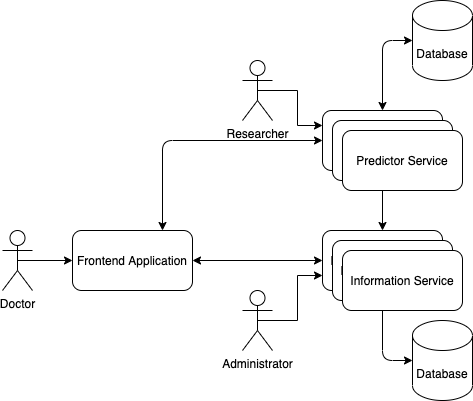
\includegraphics[scale=0.5]{figures/system-architecture}
			\fi
		\end{figure}
		Microservice pattern[\cite{newman_2020}] tries to decrease complexity and increase safety by splitting the internal logic 
		of a system into several components called 'Microservices'. Each microservice is essentially a server that handles a small 
		portion of the systems logic. As opposed to the  monolithic services, microservices have a number of advantages that made 
		them ideal for the requirements of this project such as.
		\begin{itemize}
			\item Highly maintainable and testable code
			\item Loosely coupled logic
			\item Independently deployable services
			\item No single point of failure
			\item Flexible scaleability factor
			\item Enchanced security
		\end{itemize}
		\subsection{Maintainability}
			By implementing our system using microservices[\cite{newman_2020}], we effectively separate the complex 
			logic of our system into different services. This separation of complexity leads to several elementary and 
			easily testable and maintainable entities. This brings down the maintenance costs.
		\subsection{Loosely coupled logic}
			Microservices ideally are loosely coupled. That means that changes tend to remain local to one microservice and do 
			not span multiple ones. In case that the requirements change and new features are needed, the features will not affect 
			a significant part of the code. This translates more negligible probability of occurring bugs and errors.
		\subsection{Indepedently deployable services}
			Using microservices gives us the advantage of deploying changes independently on the system, only on services that we need.
			This translates to fewer downtimes due to maintenance. An example of this will be a potential deployment of a new
			algorithm on the Prediction service. During the deployment of the new version of the Prediction service the system 
			will be unable to perform predictions, but the rest of the functionality will be unaffected as it lies under a different 
			microservice. With a monolith approach(all functionality in a single service), this would not be possible.
		\subsection{No single point of failure}
			Using microservices, we ensure that it will not propagate to the whole system when a failure occurs. In the hypothetical 
			scenario of a failure in the Prediction service, the rest of the system's functionality will remain intact during the 
			incident. This scenario with a monolithic architecture will bring the whole application into an unusable state.
		\subsection{Flexible scaleability factor}
			This is not sorely a feature of microservices but a combined feature brought by some additional design choices 
			from within the code itself. Both of the services are implemented using the actor model [\cite{hewitt2015actor}]. 
			The actor model allows, in combination with the microservice model, our services to act as a distributed system with 
			multiple nodes; this allows us to scale different services when demand changes dynamically and automatically, ensuring 
			the performance non-functional requirement we set back in \ref{non-functional-requirements}. An example of this can be 
			when multiple users simultaneously use the most advanced and CPU-Intensive algorithm, the ResNet(see \ref{prediction-service}). 
			If the system determines that the load is beyond some threshold, it can spin multiple instances of the same service. 
			The instances will coordinate themselfs automatically and split the work that needs to be done into equal amounts, 
			reducing the response time. This is implemented using the Heroku-autoscale feature and will be discussed in chapter \ref{backend}
		\subsection{Enchanced security}
			Having multiple and distinct microservice enhances security, as the malicious compromise of one microservice does not
			 imply the compromise of the whole system. In the hypothetical scenario of a malicious attacker may breach the 
			 Prediction Service, then the data of the Prediction Service will be at risk, but not the data from the Information 
			 System and vice versa.
	\section{Frontend Web App}
		The Frontend component has the responsibility of being the edge in our system.
		\begin{figure}[H]
			\iftrue
			\caption{Frontend Application}
			\centering
			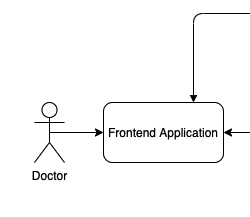
\includegraphics[scale=0.5]{figures/frontend}
			\fi
		\end{figure}
		Every action from our end-users, will be channeled through the frontend application. Our frontend is a web-based application(for 
		more information please see \ref{frontend}) and handles the application infastructure via a well designed stateful[\cite{session-rfc6265}],
		Json-based[\cite{json-rfc7159}] Https[\cite{rfc2818}] RESTFull[\cite{restful-rfc7231}]
		protocol (for more information please see chapter \ref{API}).
	\section{Backend}
		The backend services are the backbone of our application. They handle all the logic behind the application, from the saving 
		and retrieval of patients, scans, images, and notifications, to the prediction and classification of the ultrasound images. 
		There are two services with distinct areas of interest and different purposes, the Information Backend(also known as 
		'Information Service' to the simplified diagrams) and Task Backend(Also known as Predictor Service).
		\subsection{Information Backend}
			\begin{figure}[H]
				\iftrue
				\caption{Information Service}
				\centering
				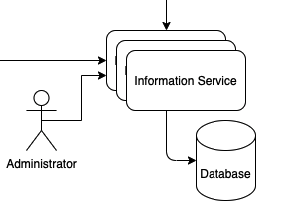
\includegraphics[scale=0.5]{figures/infobe}
				\fi
			\end{figure}
			The Information Backend has the responsibility to perform all the logic apart from the prediction itself. It
			 includes the functionality of keeping the associations of Patients, Scans, and the information composing those 
			 entities. It also includes the notification system and authentication services. Finally, it includes a small 
			 application for use by the NOC\footnote{Network operations center}  for administrator purposes.
		\subsection{Task Backend}
			\begin{figure}[H]
				\iftrue
				\caption{Predictor Service}
				\centering
				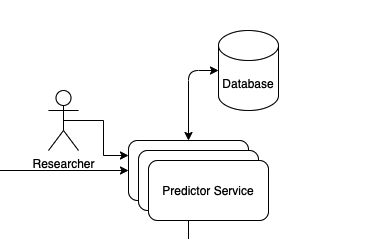
\includegraphics[scale=0.5]{figures/taskbe}
				\fi
			\end{figure}
			The Task Backend has the responsibility of performing the predictions based on the received ultrasound scan images. 
			After completing a prediction, Task Backend should communicate with Information Backend to inform the user about the 
			completion of the scan. Finally, it includes a small application for use by the researcher to gather the data and the 
			feedback from the end-users.
	
		
				
					
			
		
	
